\chapter{Реализация программы}
\section{Предварительная работа с динамической библиотекой}\label{base.txt}
Для того, чтобы при изменении динамической библиотеки не нужно было менять код программы было сделано следующее. В корневом каталоге с файлами, необходимыми для создания сервера, создаётся текстовый файл base.txt. Содержание файла формируется из информации о функциях, заявленных в динамической библиотеке. Каждая функция записывается в текстовый файл  следующим образом:
\begin{lstlisting}[numbers=none, language=bash]
"function name","return type","var's type",["var's type", [...]],
\end{lstlisting}
Сначала записывается имя функции, потом тип возвращаемого значения, далее перечисляются типы передаваемых переменных в фукнцию в том порядке, в котором они идёт в ней. В конце записи ставится запятая.
Следующая функция записывается со следующей строки.
После того как все функции описаны, на следующей строке записывается имя динамической библиотеки без расширения. После имени никаких символов не ставится. К созданной динамической библиотеке (см. пункт ~\ref{CreationDynLib}) файл base.txt будет выглядеть следующим образом:
 \lstinputlisting[frame=shadowbox, 
   emph={forsuffixes,text,bpath},emphstyle={\color{red}},
   emph={[2]fill,unfill},emphstyle={[2]\bfseries\underbar}
 ]{../base.txt}
В пункте ~\ref{projectStructure} описано, как используется этот файл.
\section{Оформление запроса}
Flash-приложение посылает запрос на сервер. Сервер разбирает этот запрос, выполняет нужную функцию из динамической библиотеке, и посылает результат выполнения ответов. Разберем, как организовать запрос на примере:
\begin{lstlisting}[numbers=none, language=bash]
"http://127.0.0.1:8888/>?int=subtraction+float=123.3+int=1"
\end{lstlisting}
\begin{itemize}
   \item http://127.0.0.1:8888/ - сайт, куда посылается запрос с портом, который прослушивает сервер;
   \item >? - данный символ указывает серверу на то, что этот запрос - это запрос на выполнение функции из подгружаемой динамической библиотеки;
  \item int=subtraction - тип возвращаемого значения и имя функции;
  \item float=123.3 - тип передаваемого параметра и его значения;
\end{itemize}
Между параметрами и описанием функции ставится \textbf{+}. Все передаваемые параметры должны быть перечислены строго в том порядке, в котором они заданы в функции из динамической библиотеки. Тип параметров должны в точности совпадать с типами передаваемых переменных, объявленных в функции.
На данном этапе разработки при неправильно созданном запросе, сервер пытается найти функцию с такими параметрами и, не находя её, аварийно завершает работу.
Существует следующие варианты того, как будет вести себя сервер при неверном запросе:
\begin{itemize}
  \item Пропускать данный запрос, не уведомляя об ошибке запроса.
  \item Возвращать ошибку.
\end{itemize}
Для программиста, который пишет Flash-программу, если он неверно задаёт запрос, для отладки важно, чтобы ему возвращалась ошибка, с указанием о том, какой запрос был создан неправильно. Поэтому выбран второй вариант. При этом важно сделать так, чтобы Flash-программисту было легко понять какой из запросов выдал ошибку, а также охрактеризовать тип ошибки, предложив пути решения. Данная проблема будет решена в следующих версиях моего проекта.
\section{Структура проекта}\label{projectStructure}
Весь проект делится на 2 части:
\begin{itemize}
  \item  Написать сервер, работающий с динамической библиотекой.
  \item Написать функцию в Flash для работы с запросом
\end{itemize}
\subsection{Серверная часть}\label{ServerPart}
Для серверной части написано три скрипта:
\begin{itemize}
  \item  http.js - Создание сервера;
  \item  readRequest.js - Разбор полученного запроса;
  \item text.js - Инициализация динамической библиотеки.
\end{itemize}
В text.js написана функция, которая на основе файла base.txt (см пункт ~\ref{base.txt}) подключает динамическую библиотеку. В readRequest.js написаны две функции. Функция GetReturnType(text) - возвращает тип возвращаемого значения функции. Функция Search(text, way) - возвращает массив, при этом если в параметр way указать значение "type", то массив будет состоять из типов передаваемых параметров. Если же передать "value" - массив значений, которые нужно передать в качестве параметров функции.
Рассмотрим работу библиотеки node-ffi на примере нашего проекта (см. ~\ref{text.js}).
 \lstinputlisting[frame=shadowbox,
   emph={forsuffixes,text,bpath},emphstyle={\color{red}},
   emph={[2]fill,unfill},emphstyle={[2]\bfseries\underbar}, caption=Код text.js. Инициализация динамической библиотеки, label={text.js}
 ]{../text.js}

Следующие строки подключают библиотеки для работы с динамическими библиотеками и для работы с файлами соответственно:
 \lstinputlisting[firstline =1, lastline=2,
   emph={forsuffixes,text,bpath},emphstyle={\color{red}},
   emph={[2]fill,unfill},emphstyle={[2]\bfseries\underbar}, 
 ]{../text.js}
В данном скрипте функция DynLib() формирует объект StructForLib для выгрузки из динамической библиотеки функций. Рис. ~\ref{StructForLib}показывает, как выглядит StructForLib перед выгрузкой из тестовой динамической библиотеки:
\begin{figure}[!ht]
	\begin{center}
		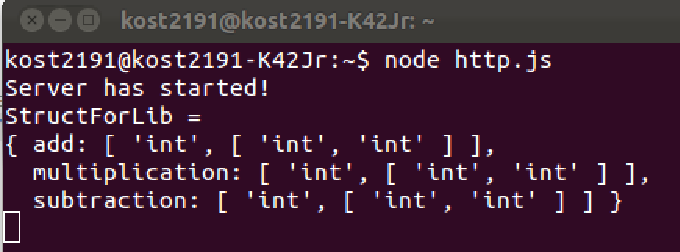
\includegraphics[width=11cm]{StructForLib}
	\end{center}
	\caption{Параметр для передачи в Library из node-ffi}
	\label{StructForLib}
\end{figure}
После того, как StructForLib был сформирован, по нему создается объект lib1 с методами, являющимися функциями динамической библиотеки:
 \lstinputlisting[firstline =40, lastline=40,
   emph={forsuffixes,text,bpath},emphstyle={\color{red}},
   emph={[2]fill,unfill},emphstyle={[2]\bfseries\underbar}, 
 ]{../text.js}
После этого в объекте lib1 станут достпуны методы: add(int, int), multiplication(int, int), subtraction(int, int).
Каждый раз при обработке запроса из lib1 будет вызываться метод, который был запрошен Flash-приложением.
 \lstinputlisting[frame=shadowbox,
   emph={forsuffixes,text,bpath},emphstyle={\color{red}},
   emph={[2]fill,unfill},emphstyle={[2]\bfseries\underbar}, caption=Код http.js. Сервер, label={http.js}
 ]{../http.js}
Сначала подключаются скрипты text.js, readRequest.js. Далее вызывается функция инициализации из text.js. После этого создается сервер, слушающий порт 8888. В котором каждый запрос с \textbf{>} обрабатывается и вызывается соответствующая функция, после чего сервер отправляет ответ, возвращаемый данной функцией. 

Строки кода 23-31 переводят уже обработанный запрос в созданный на этапе инициализации метод (его вызов записывается в переменную типа String), взятый из динамической библиотеки. В него передаются аргументы из запроса. Далее функцией eval вызывается метод, записанный в строковой переменной. Таким образом может быть вызвана любая функция из динамической библиотеки.
\subsection{Клиентская часть}
Клиентом у нас в данном случае является приложение, написанно на ActionScript. При настройках Flash по умолчанию, он не может отправлять и получать данный с локальных серверов. Так как наш сервер поднимается локально, значит нужно поменять настройки flash. Рассмотрим типы изолированной программной среды безопасности, в которой работает вызывающий файл.
\begin{itemize}
  \item REMOTE: этот файл загружается с URL-адреса в Интернете и используется в соответствии с правилами изолированной программной среды на основе домена;
  \item LOCAL\_WITH\_FILE: этот файл является локальным файлом, не является доверенным для пользователя и не публиковался с сетевым наименованием. Файл может считывать информацию из локальных источников данных, но не может обмениваться данными через Интернет;
  \item LOCAL\_WITH\_NETWORK: этот SWF-файл является локальным файлом, не является доверенным для пользователя и публиковался с сетевым наименованием. SWF-файл может обмениваться данными через Интернет, но не может считывать информацию из локальных источников данных;
  \item LOCAL\_TRUSTED: этот SWF-файл является локальным файлом, пользователь сделал его доверенным с помощью диспетчера настроек проигрывателя Flash Player или файла конфигурации FlashPlayerTrust. Файл может считывать информацию из локальных источников данных и обмениваться данными через Интернет;
  \item APPLICATION: файл работает в приложении AIR и был установлен с пакетом (файлом AIR) для этого приложения. По умолчанию файлы в изолированной программной среде безопасности приложения AIR могут выполнять перекрестные сценарии с любым файлом из любого домена (в то время как файлы за ее пределами могут не иметь разрешения на выполнение перекрестных сценариев с файлом AIR). По умолчанию файлы в изолированной программной среде безопасности приложения AIR могут загружать содержимое и данные из любого домена. 
\end{itemize}

В случае работы программиста используется FlashPlayerDebugger из Flex SDK. Он позволяет эффективно отлаживать программу, в её теле ставить breakpoint'ы а также использовать функцию trace(), выводящую в консоль IntelliJ IDEA тот параметр, который мы передали в trace().
Для смены настроек изолированной среды, нужно перейти в папку с используемым Flash Player'ом и вызвать настройки. Выбрать в настройках изолированной среды тип LOCAL\_TRUSTED и сохранить изменения.

Функция, нужная для работы программиста, представлена в листинге ~\ref{asFunc}.
\begin{lstlisting}[frame=shadowbox, language=bash,   emph={forsuffixes,text,bpath},emphstyle={\color{red}},
   emph={[2]fill,unfill},emphstyle={[2]\bfseries\underbar}, caption=Функция для Flash-приложения, label=asFunc]
    public function UrlConnect():void{
        var FuncName = "multiplication";
        var Rtype = "int";
        var a = 1;
        var b = 2;
        SendRequest(FuncName, Rtype, [a, b]);
    }

    public function SendRequest(fname: String, Rtype: String, vars: Array){
        var Rurl = "http://127.0.0.1:8888/>?" + Rtype + "=" + fname + "+";
        var i;
        for (i=0; i< vars.length; i++) {
            Rurl = Rurl + typeof(vars[i]) + "=" + vars[i];
            if (i < vars.length - 1) {
                 Rurl = Rurl + "+";
            }
        }
        trace(Rurl);
        loader.dataFormat = URLLoaderDataFormat.TEXT;
        loader.addEventListener(Event.COMPLETE, loaderHandler);
        loader.load(new URLRequest(Rurl));
    }
    public function loaderHandler(event:Event):void{

        trace(loader.data);
    }
\end{lstlisting}
Программисту для получения результата достаточно передать имя функции, тип возвращаемого значения, а также массив из аргументов. Пример этого описан в функции UrlConnect() листинга ~\ref{asFunc}. Требования к аргуменая функции SendRequest(..):
\begin{itemize}
	\item Имя функции должно присутствовать в динамической библиотеке;
	\item Тип возвращаемого значение должен соответствовать типу возвращаемого значения в функции динамической библиотеки;
	\item Аргументы функции (массив vars) должны быть указаны в правильном порядке и соответствовать типам аргументов соответствующей функции из динамической библиотеки.
\end{itemize}


